% GNUPLOT: LaTeX picture with Postscript
\begingroup
  \makeatletter
  \providecommand\color[2][]{%
    \GenericError{(gnuplot) \space\space\space\@spaces}{%
      Package color not loaded in conjunction with
      terminal option `colourtext'%
    }{See the gnuplot documentation for explanation.%
    }{Either use 'blacktext' in gnuplot or load the package
      color.sty in LaTeX.}%
    \renewcommand\color[2][]{}%
  }%
  \providecommand\includegraphics[2][]{%
    \GenericError{(gnuplot) \space\space\space\@spaces}{%
      Package graphicx or graphics not loaded%
    }{See the gnuplot documentation for explanation.%
    }{The gnuplot epslatex terminal needs graphicx.sty or graphics.sty.}%
    \renewcommand\includegraphics[2][]{}%
  }%
  \providecommand\rotatebox[2]{#2}%
  \@ifundefined{ifGPcolor}{%
    \newif\ifGPcolor
    \GPcolorfalse
  }{}%
  \@ifundefined{ifGPblacktext}{%
    \newif\ifGPblacktext
    \GPblacktexttrue
  }{}%
  % define a \g@addto@macro without @ in the name:
  \let\gplgaddtomacro\g@addto@macro
  % define empty templates for all commands taking text:
  \gdef\gplbacktext{}%
  \gdef\gplfronttext{}%
  \makeatother
  \ifGPblacktext
    % no textcolor at all
    \def\colorrgb#1{}%
    \def\colorgray#1{}%
  \else
    % gray or color?
    \ifGPcolor
      \def\colorrgb#1{\color[rgb]{#1}}%
      \def\colorgray#1{\color[gray]{#1}}%
      \expandafter\def\csname LTw\endcsname{\color{white}}%
      \expandafter\def\csname LTb\endcsname{\color{black}}%
      \expandafter\def\csname LTa\endcsname{\color{black}}%
      \expandafter\def\csname LT0\endcsname{\color[rgb]{1,0,0}}%
      \expandafter\def\csname LT1\endcsname{\color[rgb]{0,1,0}}%
      \expandafter\def\csname LT2\endcsname{\color[rgb]{0,0,1}}%
      \expandafter\def\csname LT3\endcsname{\color[rgb]{1,0,1}}%
      \expandafter\def\csname LT4\endcsname{\color[rgb]{0,1,1}}%
      \expandafter\def\csname LT5\endcsname{\color[rgb]{1,1,0}}%
      \expandafter\def\csname LT6\endcsname{\color[rgb]{0,0,0}}%
      \expandafter\def\csname LT7\endcsname{\color[rgb]{1,0.3,0}}%
      \expandafter\def\csname LT8\endcsname{\color[rgb]{0.5,0.5,0.5}}%
    \else
      % gray
      \def\colorrgb#1{\color{black}}%
      \def\colorgray#1{\color[gray]{#1}}%
      \expandafter\def\csname LTw\endcsname{\color{white}}%
      \expandafter\def\csname LTb\endcsname{\color{black}}%
      \expandafter\def\csname LTa\endcsname{\color{black}}%
      \expandafter\def\csname LT0\endcsname{\color{black}}%
      \expandafter\def\csname LT1\endcsname{\color{black}}%
      \expandafter\def\csname LT2\endcsname{\color{black}}%
      \expandafter\def\csname LT3\endcsname{\color{black}}%
      \expandafter\def\csname LT4\endcsname{\color{black}}%
      \expandafter\def\csname LT5\endcsname{\color{black}}%
      \expandafter\def\csname LT6\endcsname{\color{black}}%
      \expandafter\def\csname LT7\endcsname{\color{black}}%
      \expandafter\def\csname LT8\endcsname{\color{black}}%
    \fi
  \fi
    \setlength{\unitlength}{0.0500bp}%
    \ifx\gptboxheight\undefined%
      \newlength{\gptboxheight}%
      \newlength{\gptboxwidth}%
      \newsavebox{\gptboxtext}%
    \fi%
    \setlength{\fboxrule}{0.5pt}%
    \setlength{\fboxsep}{1pt}%
\begin{picture}(8062.00,10080.00)%
      \csname LTb\endcsname%
      \put(4031,9860){\makebox(0,0){\strut{}}}%
    \gplgaddtomacro\gplbacktext{%
      \csname LTb\endcsname%
      \put(550,7013){\makebox(0,0)[r]{\strut{}$2$}}%
      \put(550,7443){\makebox(0,0)[r]{\strut{}$3$}}%
      \put(550,7874){\makebox(0,0)[r]{\strut{}$4$}}%
      \put(550,8304){\makebox(0,0)[r]{\strut{}$5$}}%
      \put(550,8734){\makebox(0,0)[r]{\strut{}$6$}}%
      \put(550,9165){\makebox(0,0)[r]{\strut{}$7$}}%
      \put(550,9595){\makebox(0,0)[r]{\strut{}$8$}}%
      \put(682,6793){\makebox(0,0){\strut{}$390$}}%
      \put(1317,6793){\makebox(0,0){\strut{}$400$}}%
      \put(1952,6793){\makebox(0,0){\strut{}$410$}}%
      \put(2586,6793){\makebox(0,0){\strut{}$420$}}%
      \put(3221,6793){\makebox(0,0){\strut{}$430$}}%
      \put(3856,6793){\makebox(0,0){\strut{}$440$}}%
      \put(4491,6793){\makebox(0,0){\strut{}$450$}}%
      \put(5126,6793){\makebox(0,0){\strut{}$460$}}%
      \put(5761,6793){\makebox(0,0){\strut{}$470$}}%
      \put(6395,6793){\makebox(0,0){\strut{}$480$}}%
      \put(7030,6793){\makebox(0,0){\strut{}$490$}}%
      \put(7665,6793){\makebox(0,0){\strut{}$500$}}%
    }%
    \gplgaddtomacro\gplfronttext{%
      \csname LTb\endcsname%
      \put(176,8304){\rotatebox{-270}{\makebox(0,0){\strut{}  }}}%
    }%
    \gplgaddtomacro\gplbacktext{%
      \csname LTb\endcsname%
      \put(550,3726){\makebox(0,0)[r]{\strut{}$2$}}%
      \put(550,4157){\makebox(0,0)[r]{\strut{}$3$}}%
      \put(550,4587){\makebox(0,0)[r]{\strut{}$4$}}%
      \put(550,5018){\makebox(0,0)[r]{\strut{}$5$}}%
      \put(550,5448){\makebox(0,0)[r]{\strut{}$6$}}%
      \put(550,5879){\makebox(0,0)[r]{\strut{}$7$}}%
      \put(550,6309){\makebox(0,0)[r]{\strut{}$8$}}%
      \put(682,3506){\makebox(0,0){\strut{}$390$}}%
      \put(1317,3506){\makebox(0,0){\strut{}$400$}}%
      \put(1952,3506){\makebox(0,0){\strut{}$410$}}%
      \put(2586,3506){\makebox(0,0){\strut{}$420$}}%
      \put(3221,3506){\makebox(0,0){\strut{}$430$}}%
      \put(3856,3506){\makebox(0,0){\strut{}$440$}}%
      \put(4491,3506){\makebox(0,0){\strut{}$450$}}%
      \put(5126,3506){\makebox(0,0){\strut{}$460$}}%
      \put(5761,3506){\makebox(0,0){\strut{}$470$}}%
      \put(6395,3506){\makebox(0,0){\strut{}$480$}}%
      \put(7030,3506){\makebox(0,0){\strut{}$490$}}%
      \put(7665,3506){\makebox(0,0){\strut{}$500$}}%
    }%
    \gplgaddtomacro\gplfronttext{%
      \csname LTb\endcsname%
      \put(176,5017){\rotatebox{-270}{\makebox(0,0){\strut{}Absorption
            cross section [$10^{-19}$ \si{\square\centi\meter}]}}}%
    }%
    \gplgaddtomacro\gplbacktext{%
      \csname LTb\endcsname%
      \put(682,704){\makebox(0,0)[r]{\strut{}$-3$}}%
      \put(682,1090){\makebox(0,0)[r]{\strut{}$-2$}}%
      \put(682,1477){\makebox(0,0)[r]{\strut{}$-1$}}%
      \put(682,1863){\makebox(0,0)[r]{\strut{}$0$}}%
      \put(682,2249){\makebox(0,0)[r]{\strut{}$1$}}%
      \put(682,2636){\makebox(0,0)[r]{\strut{}$2$}}%
      \put(682,3022){\makebox(0,0)[r]{\strut{}$3$}}%
      \put(814,484){\makebox(0,0){\strut{}$390$}}%
      \put(1437,484){\makebox(0,0){\strut{}$400$}}%
      \put(2060,484){\makebox(0,0){\strut{}$410$}}%
      \put(2682,484){\makebox(0,0){\strut{}$420$}}%
      \put(3305,484){\makebox(0,0){\strut{}$430$}}%
      \put(3928,484){\makebox(0,0){\strut{}$440$}}%
      \put(4551,484){\makebox(0,0){\strut{}$450$}}%
      \put(5174,484){\makebox(0,0){\strut{}$460$}}%
      \put(5797,484){\makebox(0,0){\strut{}$470$}}%
      \put(6419,484){\makebox(0,0){\strut{}$480$}}%
      \put(7042,484){\makebox(0,0){\strut{}$490$}}%
      \put(7665,484){\makebox(0,0){\strut{}$500$}}%
    }%
    \gplgaddtomacro\gplfronttext{%
      \csname LTb\endcsname%
      \put(176,1863){\rotatebox{-270}{\makebox(0,0){\strut{}  }}}%
      \put(4239,154){\makebox(0,0){\strut{}Wavelength [nm]}}%
    }%
    \gplbacktext
    \put(0,0){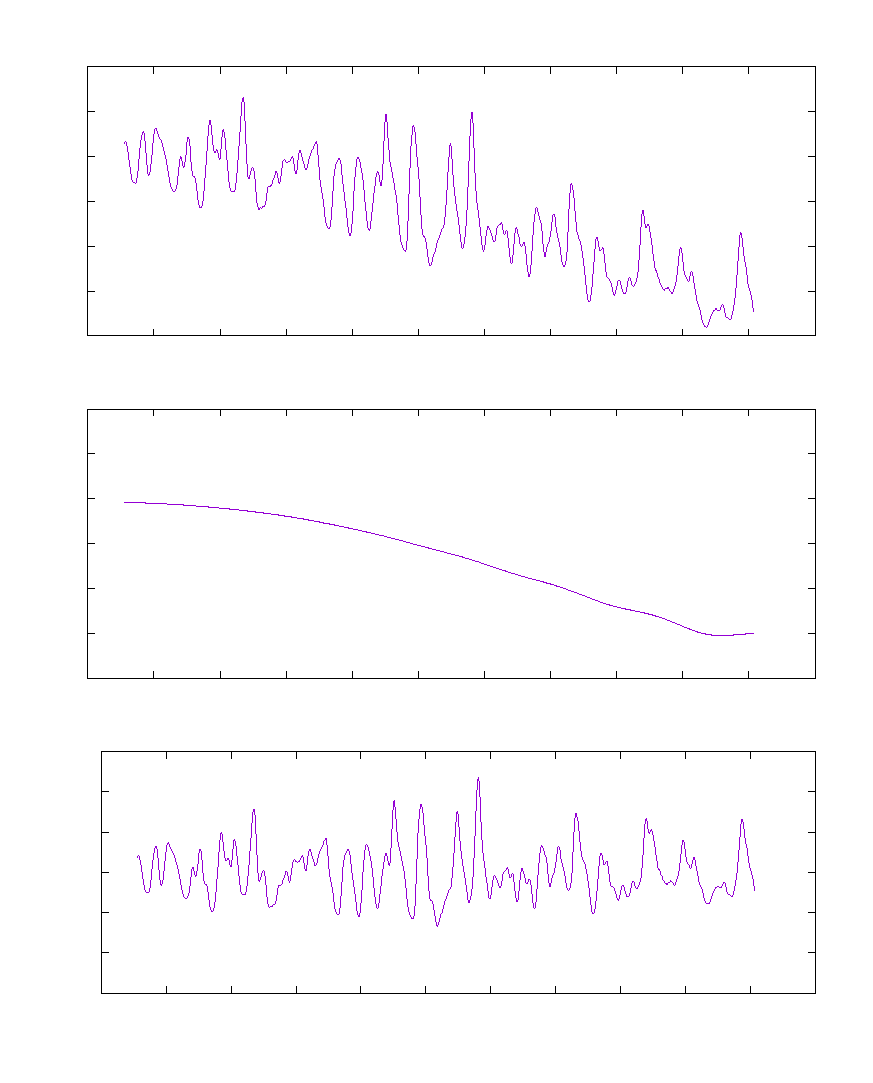
\includegraphics{../images/NO2_conv}}%
    \gplfronttext
  \end{picture}%
\endgroup
